%%
%% Copyright 2007, 2008, 2009 Elsevier Ltd
%%
%% This file is part of the 'Elsarticle Bundle'.
%% ---------------------------------------------
%%
%% It may be distributed under the conditions of the LaTeX Project Public
%% License, either version 1.2 of this license or (at your option) any
%% later version. The latest version of this license is in
%% http://www.latex-project.org/lppl.txt
%% and version 1.2 or later is part of all distributions of LaTeX
%% version 1999/12/01 or later.
%%
%% The list of all files belonging to the 'Elsarticle Bundle' is
%% given in the file `manifest.txt'.
%%

%% Template article for Elsevier's document class `elsarticle'
%% with numbered style bibliographic references
%% SP 2008/03/01

\documentclass[preprint,12pt, a4paper]{elsarticle}

%% Use the option review to obtain double line spacing
%% \documentclass[authoryear,preprint,review,12pt]{elsarticle}

%% For including figures, graphicx.sty has been loaded in
%% elsarticle.cls. If you prefer to use the old commands
%% please give \usepackage{epsfig}

%% The amssymb package provides various useful mathematical symbols
\usepackage{amssymb}
\usepackage{hyperref}
\usepackage{svg}
\setlength{\parindent}{0pt}
%% The amsthm package provides extended theorem environments
%% \usepackage{amsthm}

%% The lineno packages adds line numbers. Start line numbering with
%% \begin{linenumbers}, end it with \linenumbers}. Or switch it on
%% for the whole article with \linenumbers.
%\usepackage{lineno}

\journal{SoftwareX}

\begin{document}
\renewcommand{\labelenumii}{\arabic{enumi}.\arabic{enumii}}

\begin{frontmatter}
%% Title, authors and addresses

%% use the tnoteref command within \title for footnotes;
%% use the tnotetext command for theassociated footnote;
%% use the fnref command within \author or \address for footnotes;
%% use the fntext command for theassociated footnote;
%% use the corref command within \author for corresponding author footnotes;
%% use the cortext command for theassociated footnote;
%% use the ead command for the email address,
%% and the form \ead[url] for the home page:
%% \title{Title\tnoteref{label1}}
%% \tnotetext[label1]{}
%% \author{Name\corref{cor1}\fnref{label2}}
%% \ead{email address}
%% \ead[url]{home page}
%% \fntext[label2]{}
%% \cortext[cor1]{}
%% \address{Address\fnref{label3}}
%% \fntext[label3]{}

\title{Foruster: Live system data extraction}

%% use optional labels to link authors explicitly to addresses:
%% \author[label1,label2]{}
%% \address[label1]{}
%% \address[label2]{}

\author[label1]{Marcos Jesús Sequera Fernández}
\author[label2]{Mohammadhossein Homaei}
\author[label3]{José Carlos Sancho Núñez}
\address[label1]{marcosjesus@unex.es}
\address[label2]{mhomaein@alumnos.unex.es}
\address[label3]{jcsanchon@unex.es}

\begin{abstract}
%% Text of abstract
Foruster is a cross-platform desktop application, developed in Rust, for live-system forensic analysis. Unlike traditional tools that require system shutdown, Foruster is designed to identify and catalog files of interest on active storage volumes. Its user interface, built with the Slint framework, guides the analyst through the selection of devices, the configuration of search profiles, and the real-time visualization of results. The software features heuristic detection of anomalies, such as deceptive file extensions, and ensures the integrity of findings through cryptographic hashing, optimizing the digital forensic investigation process.
\end{abstract}

\begin{keyword}
%% keywords here, in the form: keyword \sep keyword
live-system forensics \sep forensic software \sep data extraction \sep Rust \sep digital security \sep incident response

%% PACS codes here, in the form: \PACS code \sep code

%% MSC codes here, in the form: \MSC code \sep code
%% or \MSC code \sep code (2000 is the default)

\end{keyword}

\end{frontmatter}

%\linenumbers

\section*{Metadata}
\label{}

\begin{table}[!h]
\begin{tabular}{|l|p{6.5cm}|p{6.5cm}|}
\hline
\textbf{Nr.} & \textbf{Code metadata description} & \textbf{Metadata} \\
\hline
C1 & Current code version & 1.0.0 \\
\hline
C2 & Permanent link to code/repository used for this code version & \url{https://github.com/m4rz3r0/foruster} \\
\hline
C3  & Permanent link to Reproducible Capsule & –\\
\hline
C4 & Legal Code License & GPLv3 \\
\hline
C5 & Code versioning system used & git \\
\hline
C6 & Software code languages, tools, and services used & Rust, Slint  \\
\hline
C7 & Compilation requirements, operating environments \& dependencies & Rust 1.89 \\
\hline
C8 & If available Link to developer documentation/manual & - \\
\hline
C9 & Support email for questions & marcosjesus@unex.es \\
\hline
\end{tabular}
\caption{Code metadata (mandatory)}
\label{codeMetadata}
\end{table}

\section{Motivation and significance}
Traditional digital forensic analysis, based on acquiring images of powered-off systems, presents significant challenges such as the loss of volatile evidence and the complexity of accessing encrypted volumes. Foruster addresses this problem by providing a tool for live file system analysis. Its importance lies in the ability to perform a quick and non-invasive triage, allowing access to data on unlocked encrypted volumes (such as BitLocker or LUKS) and preserving the operational state of the system.

The software contributes to the forensic discovery process by facilitating the study of volatile evidence and optimizing the initial phase of an investigation. In practical use, the analyst runs the application on the target system, selects devices and search profiles through a graphical interface, and receives real-time results, including the detection of heuristic anomalies.

\section{Software description}

Foruster is a cross-platform desktop application, developed in \textbf{Rust}, designed for live-system forensic analysis. Unlike traditional tools that require shutting down the system, Foruster is specifically designed to identify and catalog files of interest on active storage volumes. Its user interface is built with the \textbf{Slint} framework, resulting in a native application that guides the analyst through the process of selecting devices, configuring profiles, and visualizing results in real time.

\subsection{Modular Architecture and Technology Stack}

Foruster's design is based on a modular architecture implemented through a Rust \textit{workspace}, separating functionality into logical layers through different \textit{crates} to optimize maintainability and performance (see Figure~\ref{fig:arquitectura}).

At the base is the \texttt{foruster-storage} \textit{crate}, which manages the complexity of interacting with the operating system. This layer encapsulates the differences between platforms to detect and enumerate storage devices. For storage interaction on \textbf{Windows}, Foruster directly uses the native Win32 APIs (via the \texttt{windows} \textit{crate}), allowing it to query logical volumes (\texttt{FindFirstVolumeW}) and physical disks by sending I/O control codes (\texttt{DeviceIoControl} sobre rutas como \texttt{$\backslash$$\backslash$.$\backslash$PhysicalDriveX}). On \textbf{Linux} systems, the \textit{crate} interacts with the \texttt{/sys/block} and \texttt{/proc/self/mountinfo} virtual file systems to build the map of disks and partitions.

The business logic is implemented in the \texttt{analysis} and \texttt{profiling} \textit{crates}. The analysis engine runs concurrently on the \textbf{Tokio} asynchronous \textit{runtime}, using the \texttt{async-walkdir} \textit{crate} for efficient file system scanning. This engine is responsible for applying the rules of the search "Profiles" (defined in \texttt{profiling}), which are collections of criteria based on file categories, MIME types, or specific extensions.

Finally, the \texttt{api} layer acts as an intermediate bridge, transforming the data structures of the \textit{backend} into safe and easy-to-consume interfaces for the graphical user interface (\texttt{desktop}).

\begin{figure}[h!]
\centering
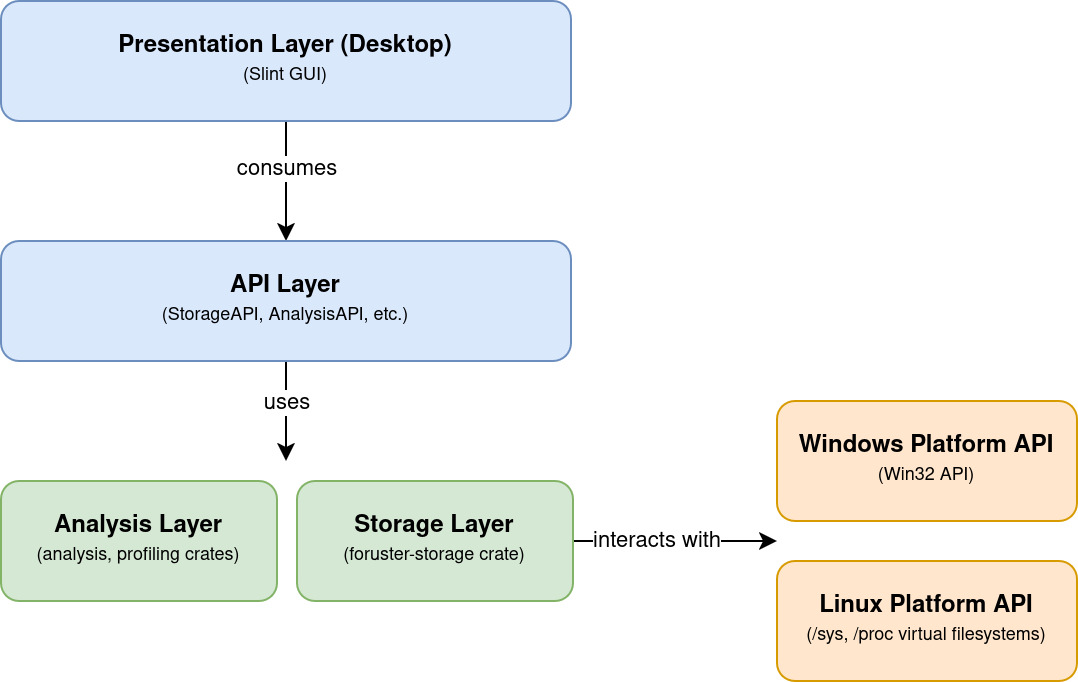
\includegraphics[width=0.8\textwidth]{resources/foruster_architecture.jpg}
\caption{Diagram of Foruster's architecture, showing its modular layers from the user interface to the interaction with the operating system.}
\label{fig:arquitectura}
\end{figure}

\subsection{Evidentiary Admissibility and Chain of Custody Compliance}

The proper extraction of file-based digital evidence requires a methodological approach that guarantees its integrity and authenticity, a fundamental principle for its evidentiary admissibility. The ISO/IEC 27037 standard provides key guidelines in this area. In live analysis scenarios ("hot work"), the methodology must minimize the footprint on the system, preserve file metadata, and ensure traceability through a robust chain of custody. Foruster has been designed to operate within this rigorous framework, structuring its functionalities around the forensic phases of identification, acquisition, preservation, and presentation.

\subsubsection{Identification and Acquisition Phase}

This phase focuses on locating and collecting potential evidence. Foruster addresses this by allowing a reproducible selection of the analysis scope, where the investigator defines the storage devices and search profiles. The analysis engine (analysis::walker) operates on the file system layer, which minimizes direct interaction with the hardware and reduces the system's footprint. This approach allows the acquisition of data from encrypted volumes (BitLocker, LUKS) that are mounted, a common scenario in active systems. Additionally, Foruster implements heuristics for identifying anomalies, such as discrepancies between the actual file type (verified using "magic numbers" with the file-format crate) and its extension, thus uncovering evidence that may have been intentionally obfuscated.

\subsubsection{Preservation and Presentation Phase}

To ensure that the evidence is not altered or contaminated, the preservation phase is critical. Foruster ensures the integrity of each identified file by generating multiple cryptographic hashes. For each relevant file, the software calculates its MD5, SHA-256, and BLAKE3 hashes. This set of hashes acts as a unique digital signature of the file's state at the exact moment of acquisition. This process is fundamental for the presentation of the evidence, as it establishes an auditable chain of custody. Any subsequent verification can recalculate these hashes to confirm that the presented evidence is an exact copy of the original.

\subsubsection{Presentation Phase}

The presentation of evidence must be clear, verifiable, and adhere to recognized standards. Foruster fulfills this phase in two ways. First, through its graphical interface, which allows the analyst a real-time visualization and filtering of the findings. Second, and more formally, by generating a final report in PDF format through the genpdfi crate. This document acts as a signed manifest of the extraction: it includes a detailed record of the operations, the analysis configuration, the characteristics of the investigated disks, and, crucially, a list of all relevant files along with their cryptographic hashes. This final report constitutes a transparent and verifiable artifact that supports the presentation of evidence in a potential judicial context.

\begin{figure}[h!]
\centering
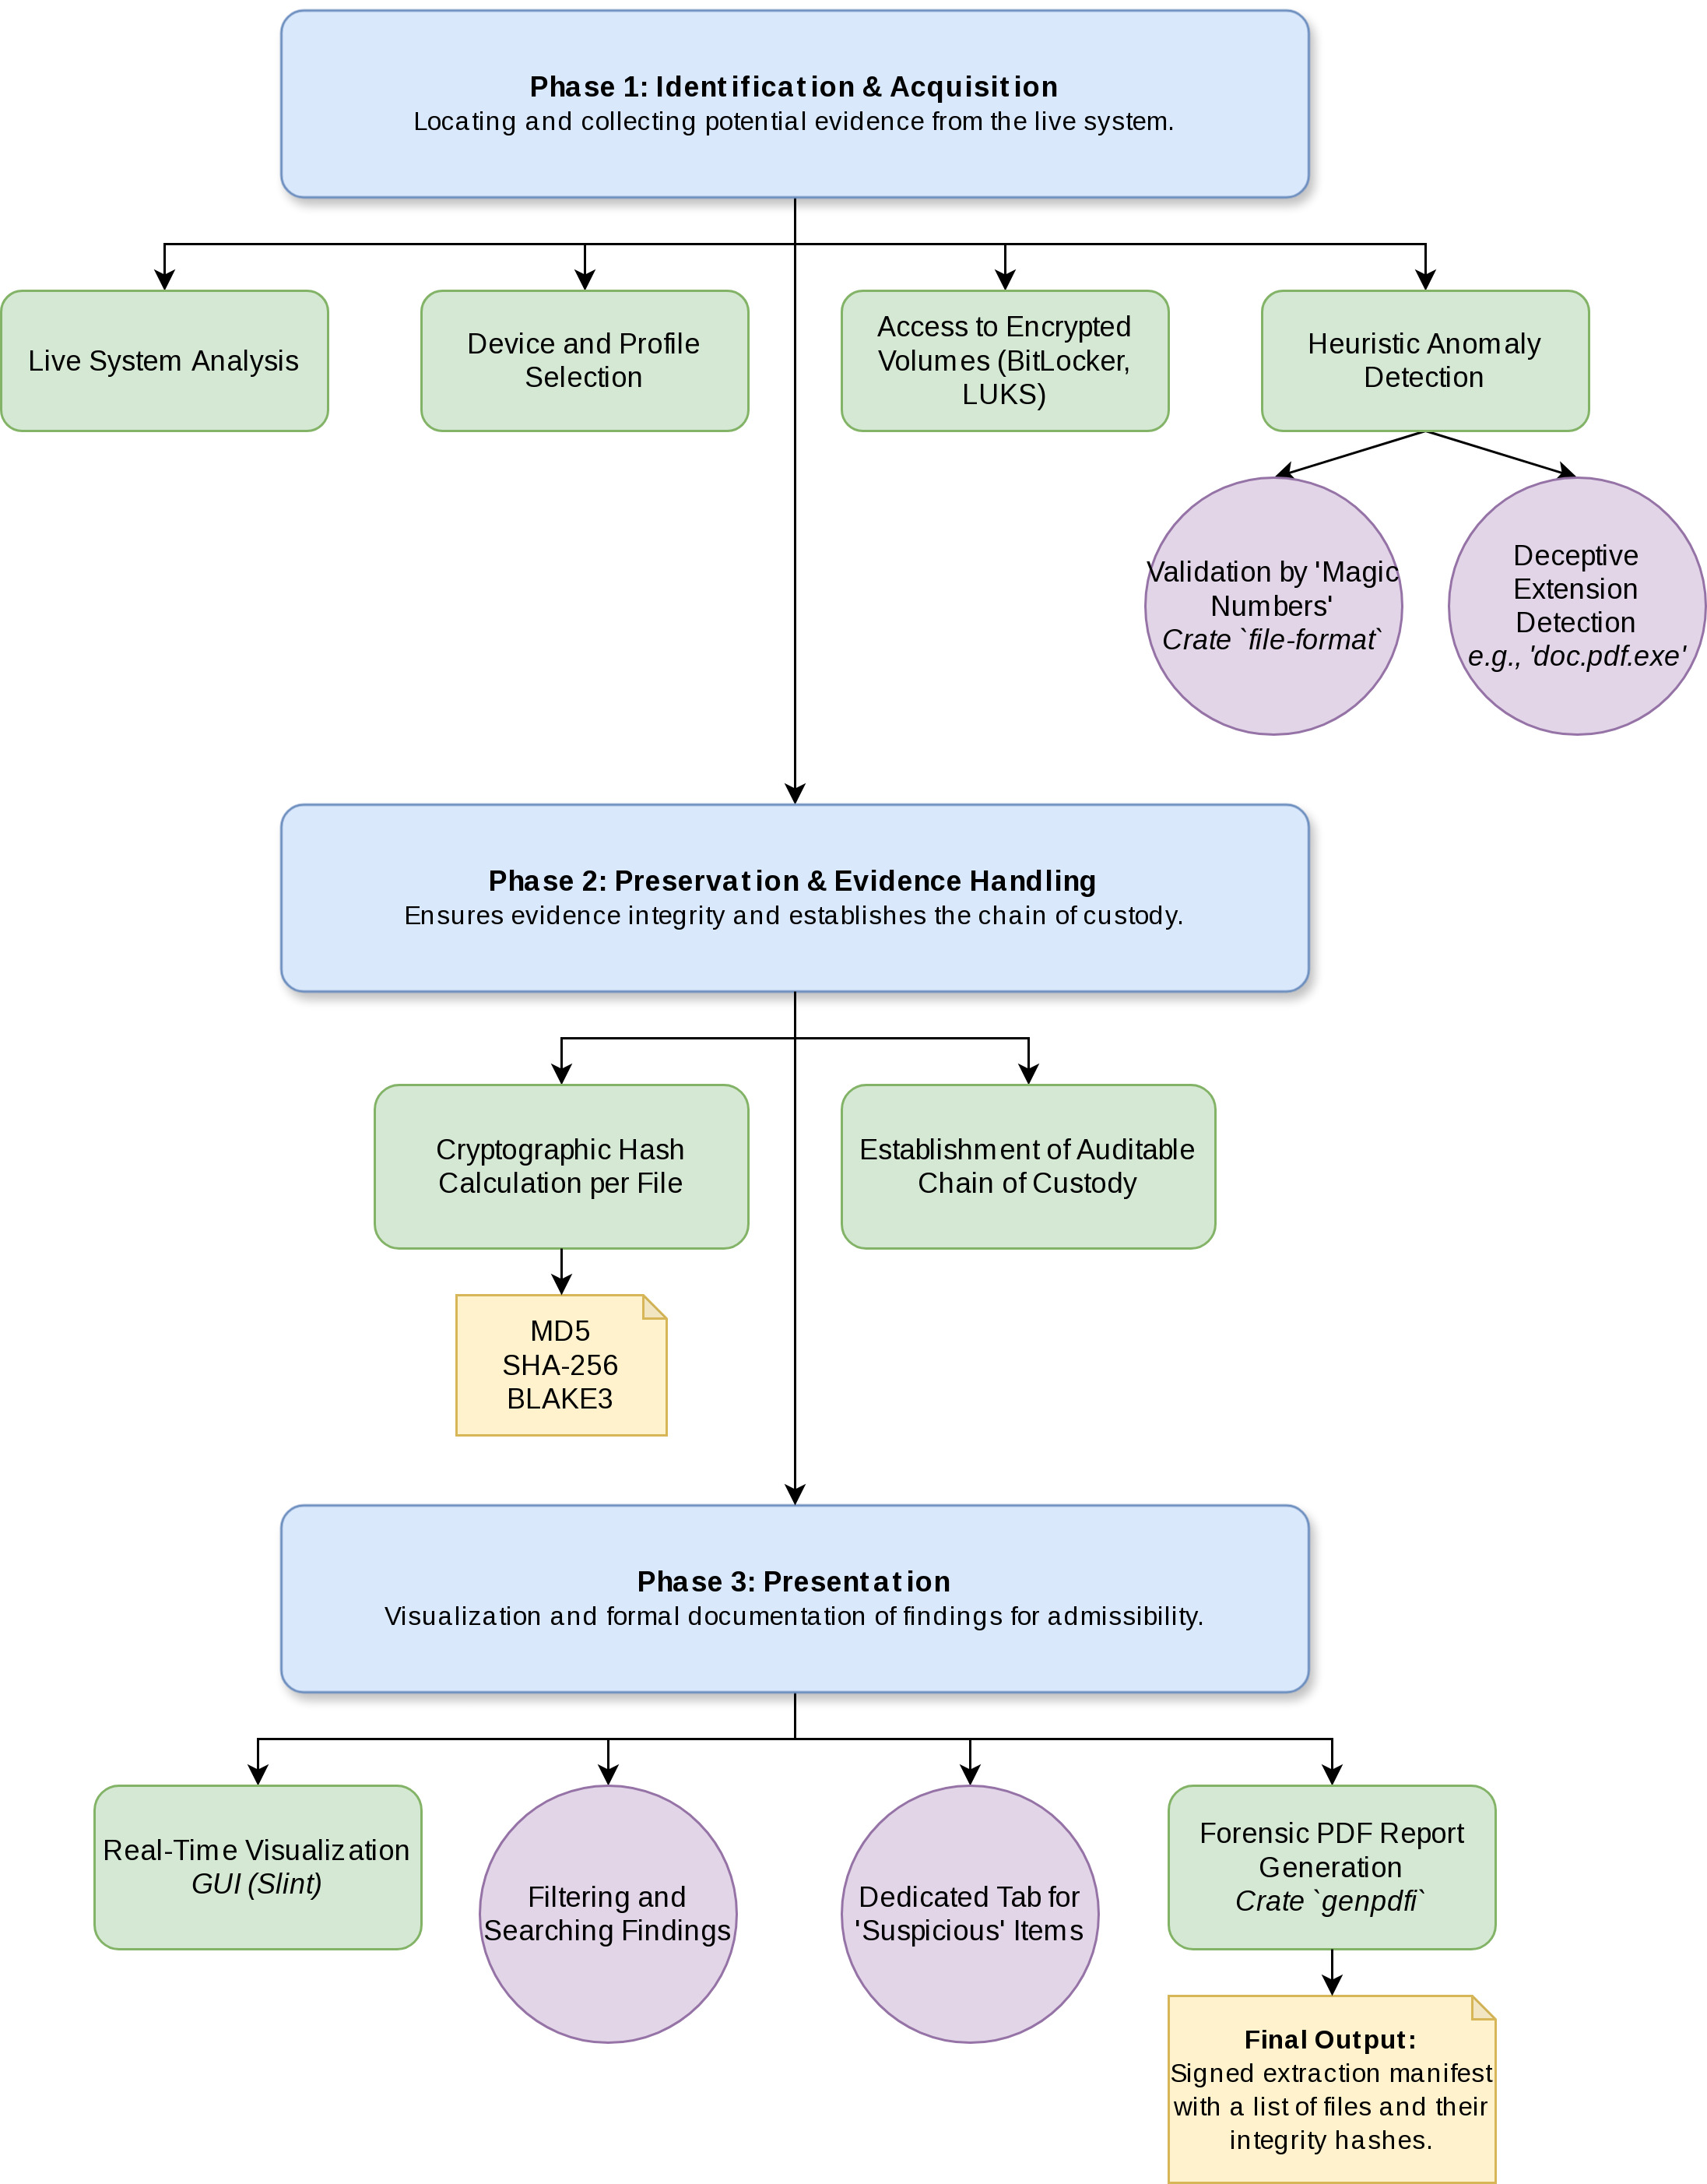
\includegraphics[width=0.8\textwidth]{resources/foruster_features.jpg}
\caption{Diagram of Foruster's features, showing its modular layers}
\label{fig:features}
\end{figure}

\section{Illustrative examples}

To demonstrate Foruster's main functions, let's consider an incident response scenario in a corporate environment. A forensic analyst needs to investigate an employee's workstation suspected of having extracted confidential information to an external storage device, all without interrupting the system's operations.

The analyst runs Foruster directly on the active system. The application immediately presents a list of connected storage devices, including the system's main disk (C:$\backslash$) and a newly connected USB drive. The analyst selects both devices for analysis. Next, the interface allows them to configure the search profiles. Since data exfiltration is suspected, they choose the predefined "Documents" and "Images" profiles, which are configured to search for common MIME types and file extensions associated with these formats.

Upon starting the analysis, the interface displays the scan's progress in real time, updating counters for analyzed files, matches found, and, crucially, suspicious files. Once the process is complete, the analyst navigates to the "Suspicious" results tab. There, they find a file named annual\_report.jpg located on the USB drive. Foruster has marked it as suspicious because, although its extension is .jpg, the validation of its content using "magic numbers" (performed by the file-format crate) has determined that it is actually a compressed file (application/zip). This finding is a high priority, as it suggests an attempt to obfuscate confidential data.

Finally, the analyst uses the export function to generate a forensic report in PDF format. This document, created by the genpdfi crate, not only summarizes the analysis statistics and the profiles used but also includes a detailed section on the suspicious findings. In this section, the file annual\_report.jpg is listed, along with the reason for suspicion (discrepancy between extension and content) and its corresponding cryptographic hashes (MD5, SHA-256, and BLAKE3), thus ensuring an auditable chain of custody and preserving the integrity of the digital evidence for further in-depth analysis.


To complement this textual description, a short demonstration video has been prepared that shows this same process in action, from device selection to the generation of the final report. The video is available as supplementary material along with this article.

\section{Impact}
The main impact of Foruster lies in its ability to shift the paradigm of digital forensic analysis, moving it from the post-mortem investigation of powered-off systems to a dynamic analysis of live systems. This capability not only improves the efficiency of existing investigations but also opens new avenues of research and modifies the daily practice of forensic analysts and incident response teams.

The availability of Foruster allows for an improved search for answers to existing research questions about the volatility of digital evidence. By operating on an active system, the software allows for the capture of the state of files at a precise moment, which facilitates comparative studies between evidence obtained live and that extracted from a traditional forensic image. This helps to quantify which artifacts are lost or altered when a system is shut down, an area of constant interest in forensic science. Additionally, the tool streamlines the triage phase of an investigation, allowing analysts to quickly determine if a system warrants a more in-depth analysis and the creation of a complete image, thus optimizing the use of time and resources.

Furthermore, the existence of Foruster raises new research questions that can be explored. For example, what is the performance impact on a host system while running a concurrent analysis with Foruster, and how can it be minimized to avoid altering the evidence? Or, can more sophisticated real-time anomaly detection heuristics be developed, based not only on metadata but also on file behavior? The use of Rust as a development language also opens a line of research on how memory safety guarantees influence the reliability and forensic soundness of software tools.

In terms of daily practice, Foruster introduces a fundamental change in an analyst's workflow. Instead of the first step being to disconnect the equipment, it is now possible to perform a non-invasive preliminary scan. This capability is especially transformative when dealing with encrypted volumes, as Foruster operates on the decrypted and mounted file system, bypassing the need for complex offline decryption processes and allowing immediate access to the data.

Since Foruster is a recently created project, its use is not yet widespread. However, as an open-source and cross-platform tool, hosted on a public GitHub repository, it is available for adoption by forensic analysts, academic researchers, and cybersecurity professionals. The publication of this article seeks to foster a community of users and contributors to drive its dissemination. Currently, its use in commercial environments is unknown, nor has it led to the creation of spin-off companies, but its open-source license (GPLv3) allows for its evaluation and integration into security consulting or incident response services.

\section{Conclusions}

\section*{Acknowledgements}
\label{}
This initiative is carried out within the framework of the funds from the Recovery, Transformation and Resilience Plan, financed by the European Union (Next Generation) - National Institute of Cybersecurity (INCIBE) in the project C108/23 "Detection of Identity Document Forgery using Computer Vision and Artificial Intelligence Techniques".

%% The Appendices part is started with the command \appendix;
%% appendix sections are then done as normal sections
%% \appendix

%% \section{}
%% \label{}

%% References:
%% If you have bibdatabase file and want bibtex to generate the
%% bibitems, please use
%%
%% \bibliographystyle{elsarticle-num}
%% \bibliography{<your bibdatabase>}

%% else use the following coding to input the bibitems directly in the
%% TeX file.

\begin{thebibliography}{00}

%% \bibitem{label}
%% Text of bibliographic item

\end{thebibliography}

\end{document}
\endinput
%%
%% End of file `SoftwareX_article_template.tex'.

%%% Local Variables:
%%% mode: latex
%%% TeX-master: t
%%% End:
